% Name: Trie
% Description: A prefix tree holding the words to, tea, ted, ten, i, in, and inn: each edge adds one letter, and a filled node marks the end of a word.
% Tags: trie, prefix tree, strings, data structures

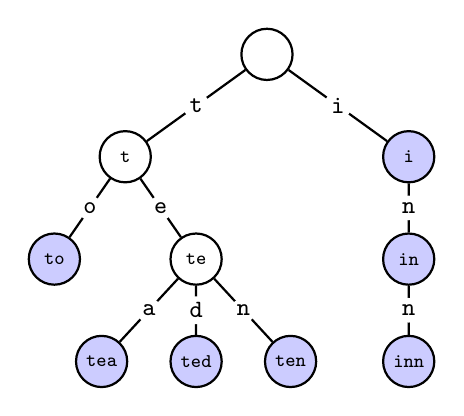
\begin{tikzpicture}[
    every node/.style={circle, draw, thick, minimum size=6.5mm, inner sep=0pt, font=\scriptsize\ttfamily},
    word/.style={fill=blue!20},
    level distance=13mm, level 1/.style={sibling distance=36mm}, level 2/.style={sibling distance=18mm}, level 3/.style={sibling distance=12mm},
    edge from parent/.style={draw, thick},
    letter/.style={draw=none, font=\small\ttfamily, fill=white, inner sep=1pt, minimum size=0pt}]
  \node {}
    child { node {t}
      child { node[word] {to} edge from parent node[letter] {o} }
      child { node {te}
        child { node[word] {tea} edge from parent node[letter] {a} }
        child { node[word] {ted} edge from parent node[letter] {d} }
        child { node[word] {ten} edge from parent node[letter] {n} }
        edge from parent node[letter] {e} }
      edge from parent node[letter] {t} }
    child { node[word] {i}
      child { node[word] {in}
        child { node[word] {inn} edge from parent node[letter] {n} }
        edge from parent node[letter] {n} }
      edge from parent node[letter] {i} };
\end{tikzpicture}
